\chapter{Verifica e validazione}
\label{cap:verifica-validazione}

\intro{In questo capitolo vengono riportati tutti i dati e le prove effettuate sul RALM per ogni modifica aggiunta}

\section{Test}
Come fonte di informazioni per il RALM sono state scelte cinque pagine di Wikipedia e sono state convertite nei formati desiderati (HTML, Pdf, Docx).
La pagine scelte sono composte di testo e altri elementi semantici, tra cui le tabelle che hanno la struttura della tabella \ref{tab:esempio-cibo} spiegata nel paragrafo \nameref{subsubsec-lin-tab}

I test sono stati effettuati tramite una valutazione umana secondo i seguenti criteri:
\begin{itemize}
    \item La risposta deve essere ben strutturata, scritta in maniera corretta e comprensibile;
    \item La risposta deve essere corretta e completa.
\end{itemize}

Sulla base di ciò a ogni risposta viene assegnato un valore tra 0 (risposta non corretta/strutturata male) e 1 (risposta corretta e strutturata correttamente)

\subsection{Domande}
Sono stati creati due set da 10 domande l'uno, le domande sono state create in maniera tale da poter interrogare il modello sui dati presenti nelle tabelle dei vari documenti:
\begin{itemize}
    \item Set di domande semplici: domande che interrogano il RALM su singole celle delle tabelle, celle che hanno la stessa intestazione o su singole righe;
    \item Set di domande complesse: domande che interrogano il RALM su diverse celle e che chiedono di fare diverse operazioni tra i dati presenti (es: somma, media).
\end{itemize}

\subsubsection{Set di domande semplici}
\begin{table}[H]
    \centering
    \begin{tabular}{|p{0.5cm} |p{2.5cm} |p{4cm}| p{4.5cm}|}
        \hline
        \textbf{N}. & \textbf{Nome pagina} & \textbf{Domanda} & \textbf{Risposta corretta} \\
        \hline
        1 & Italia & Quali sono le 3 città italiane con più abitanti? & Roma, Milano, Napoli \\
        \hline
        2 & Italia & In Italia, tra commercio, turismo e trasporti chi rappresenta un numero maggiore di imprese? & Il commercio \\
        \hline
        3 & Avanti un altro! & In quali paesi è stato esportato Avanti un altro? & Spagna, Albania, Ungheria, Vietnam, Brasile, Bulgaria, Cile, Paraguay, Canada, Turchia, Polonia, Romania \\
        \hline
        4 & Avanti un altro! & In che canale è stato trasmesso Avanti un altro? & Canale 5\\
        \hline
        5 & SPAR & In che anno è arrivato SPAR in italia? & 1959 \\
        \hline
        6 & SPAR & Quanto volume d'affari ha SPAR in Belgio & 626.307 \\
        \hline
        7 & The Space Cinema & Quante sale ha il The Space Cinema di Padova? & 14 \\
        \hline
        8 & The Space Cinema & Quanti posti a sedere ha il The Space Cinema di Parma centro & 1402 \\
        \hline
        9 & Sonic(serie) & In che anno è uscito il videogioco "Sonic Battle"? & 2003 \\
        \hline
        10 & Sonic(serie) & Dov'è apparso Tails per la prima volta? & Sonic the hedghog 2 \\
        \hline
    \end{tabular}
    \caption{Set di domande semplici poste al RALM.}
\end{table}

\subsubsection{Set di domande complesse}
\begin{table}[H]
    \centering
    \begin{tabular}{|p{0.5cm} |p{2.5cm} |p{4cm}| p{4.5cm}|}
        \hline
        \textbf{N}. & \textbf{Nome pagina} & \textbf{Domanda} & \textbf{Risposta corretta} \\
        \hline
        1 & Italia & Quali sono i comuni italiani con più di 500000 abitanti? & Roma, Milano, Napoli, Torino, Palermo e Genova \\
        \hline
        2 & Italia & Quali sono i comuni italiani che hanno più 300000 abitanti ma meno di 387843? & Bologna, Firenze, Bari, Catania \\
        \hline
        3 & Avanti un altro! & Mediamente quanti telespettatori ci sono stati per ogni edizione di avanti un altro? & circa 3.5 milioni \\
        \hline
        4 & Avanti un altro! & In quali paesi in cui è stato esportato avanti un altro è ancora in corso? & Canada, Romania \\
        \hline
        5 & SPAR & In quali paesi è arrivato SPAR dal 2000 in poi? & Russia, Mauritius, Cipro, Ucraina, Cina, Croazia \\
        \hline
        6 & SPAR & In quali paesi le strutture SPAR hanno meno di 10000 metri quadrati di superficie? & Croazia, Mauritious, Zambia,  India, Albania \\
        \hline
        7 & The Space Cinema & Quali sono i the space situati in provincia di Torino? & Beinsasco, Torino - Parco Dora \\
        \hline
        8 & The Space Cinema & Quali sono i the space con più di 13 sale? & Limena, Roma Paroc de' Medici,  Vimercate \\
        \hline
        9 & Sonic(serie) & Chi è eggman e quando ha fatto la sua prima apparizione? & Eggman è un uomo esperto di ingegneria robotica che vuole conquistare il mondo di Sonic, antagonista principale della serie. Ha fatto la sua prima apparizione in "Sonic the hedghog". \\
        \hline
        10 & Sonic(serie) & Elenca tutti i giochi mobile di Sonic dal 2015 in poi & Sonic runners, sonic dash 2: sonic boom, sonic runners adventure, sonic forces speed battle, sonic speed simulaor \\
        \hline
    \end{tabular}
    \caption{Set di domande complesse poste al RALM.}
\end{table}

Nei seguenti paragrafi vengono riportate le risposte del RALM a ogni aggiornamento significativo del codice per denotare l'effettivo miglioramento della qualità delle risposte:

\begin{enumerate}
    \item Prima versione: estrazione del contenuto semplice (senza linearizzazione delle tabelle, senza correzione del chunking e pulizia del testo);
    \item Seconda verione: estrazione del contenuto con la linearizzazione delle tabelle;
    \item Terza versione: estrazione del contenuto con la linearizzazione delle tabelle e la correzione del chunking e pulizia del testo;

\end{enumerate}


\subsection{Test sui file HTML}

\subsubsection{Prima versione - Risposte al set di domande semplici}

\begin{table}[H]
    \centering
    \begin{tabular}{|p{0.5cm} |p{6cm} |p{2cm}|}
        \hline
        \textbf{N}. & \textbf{Risposta fornita dal RALM} & \textbf{Valutazione} \\
        \hline
        1 & Roma, Milano e Napoli sono le tre città italiane con più abitanti. & 1 \\
        \hline
        2 & Il settore che presenta più imprese nel terziario italiano è il settore dei servizi. & 0 \\
        \hline
        3 & Avanti un altro! è stato esportato in Spagna, Albania, Ungheria, Vietnam, Brasile, Paraguay, Cile, Bulgaria, Canada, Turchia, Polonia e Romania. & 1 \\
        \hline
        4 & Avanti un altro è stato trasmesso sul canale 5. & 1 \\
        \hline
        5 & SPAR è arrivato in Italia nel 1959. & 1 \\
        \hline
        6 &  SPAR in Belgio & 0 \\
        \hline
        7 & Il the space di Padova ha 14 sale & 1 \\
        \hline
        8 & Il The Space di Parma Centro ha 7 sale e 1402 posti a sedere & 1 \\
        \hline
        9 & Il videogioco Sonic Battle è stato pubblicato da Sega nel 2003. & 1 \\
        \hline
        10 & Tails è un compagno di Sonic che appare per la prima volta in Sonic the Hedgehog 2 nel 1992. & 1 \\
        \hline
    \end{tabular}
    \caption{Risposte al set di domande semplici date dalla prima versione del RALM (File HTML).}
\end{table}

\textbf{Correttezza:} 8/10

\subsubsection{Prima versione - Risposte al set di domande complesse}

\begin{table}[H]
    \centering
    \begin{tabular}{|p{0.5cm} |p{6cm} |p{2cm}|}
        \hline
        \textbf{N}. & \textbf{Risposta fornita dal RALM} & \textbf{Valutazione} \\
        \hline
        1 & Palermo, Cagliari, Trento, Venezia, Trieste, Bologna, Firenze, Perugia, Ancona, Roma, Napoli, Bari, Potenza, Catanzaro, Matera, Belluno & 0 \\
        \hline
        2 & Napoli, Palermo, Genova, Bologna, Firenze e Bari. & 0 \\
        \hline
        3 & In media si contano 3.995.000 spettatori per edizione. & 0 \\
        \hline
        4 & Il programma "Avanti un altro!" è ancora in corso in Italia, mentre negli altri paesi in cui è stato esportato è chiuso. & 0 \\
        \hline
        5 & SPAR è arrivata in Belgio, Danimarca, Francia, Germania, Irlanda, Italia, Lituania, Paesi Bassi, Polonia, Regno Unito, Russia, Sudafrica, Spagna, Svizzera, Ungheria, Zimbabwe. & 0 \\
        \hline
        6 & SPAR è presente in Croazia, Slovenia, Austria, Germania, Regno Unito, Italia, Sudafrica, Norvegia, Giappone, Cina e Croazia. & 0 \\
        \hline
        7 & The Space Cinema è una catena di cinema presente in provincia di Torino. Ha 8 sale e 1295 posti a sedere. & 0 \\
        \hline
        8 & The Space Cinema è una delle catene di cinema più grandi in Italia, con 34 diverse strutture e 347 sale.  & 0 \\
        \hline
        9 & Eggman è un personaggio che è appena comparso nella serie Sonic. È uno scienziato malvagio che cerca di conquistare il mondo. & 0 \\
        \hline
        10 & Sonic mobile games from 2015 onwards: Sonic Jump (2015), Sonic Dash (2013), Sonic Jump Fever (2014), Sonic Runners (2015), Sonic Dash 2: Sonic Boom (2015), Sonic Runners Adventure (2017), Sonic Forces: Speed Battle (2017), Sonic Speed Simulator (2022) & 0 \\
        \hline
    \end{tabular}
    \caption{Risposte al set di domande complesse date dalla prima versione del RALM (File HTML).}
\end{table}

\textbf{Correttezza:} 0/10

\subsubsection{Seconda versione - Risposte al set di domande semplici}

\begin{table}[H]
    \centering
    \begin{tabular}{|p{0.5cm} |p{6cm} |p{2cm}|}
        \hline
        \textbf{N}. & \textbf{Risposta fornita dal RALM} & \textbf{Valutazione} \\
        \hline
        1 & Roma, Milano e Napoli sono le prime tre città italiane per popolazione. & 1 \\
        \hline
        2 & Il commercio è il settore che presenta più imprese in Italia, seguito da turismo, trasporti e logistica, e altri servizi. & 1 \\
        \hline
        3 & Avanti un altro! è stato esportato in Spagna, Albania, Ungheria, Vietnam, Brasile, Paraguay, Cile, Bulgaria, Canada, Turchia, Polonia e Romania. & 1 \\
        \hline
        4 & Avanti un altro è stato trasmesso sul canale 5. & 1 \\
        \hline
        5 & SPAR è arrivato in Italia nel 1959. & 1 \\
        \hline
        6 & SPAR ha un volume d'affari di 626.307 migliaia di € in Belgio. & 1 \\
        \hline
        7 & Il the space di Padova ha 14 sale & 1 \\
        \hline
        8 & The Space Cinema di Parma Centro ha 1402 posti a sedere. & 1 \\
        \hline
        9 & Il videogioco Sonic Battle è uscito nel 2003. & 1 \\
        \hline
        10 & Tails ha fatto la sua prima apparizione in Sonic the Hedgehog 2 (8-bit) nel 1992. Da allora, è apparso in un totale di 56 giochi. & 1 \\
        \hline
    \end{tabular}
    \caption{Risposte al set di domande semplici date dalla seconda versione del RALM (File HTML).}
\end{table}

\textbf{Correttezza:} 10/10

\subsubsection{Seconda versione - Risposte al set di domande complesse}

\begin{table}[H]
    \centering
    \begin{tabular}{|p{0.5cm} |p{6cm} |p{2cm}|}
        \hline
        \textbf{N}. & \textbf{Risposta fornita dal RALM} & \textbf{Valutazione} \\
        \hline
        1 & Le città italiane con più di 500.000 abitanti sono Milano, Roma, Torino, Palermo, Napoli e Genova. & 1 \\
        \hline
        2 & Bologna, Firenze, Bari, Catania & 1 \\
        \hline
        3 & Non è chiaro quanto sia l'edizione di Avanti un altro, ma si stima che ci siano stati 3 milioni di telespettatori per edizione. & 0 \\
        \hline
        4 & Il gioco "Avanti un altro!" è stato esportato in Spagna, Albania, Ungheria, Vietnam, Brasile, Paraguay, Cile e Bulgaria. & 0 \\
        \hline
        5 & I Paesi in cui è arrivato SPAR dal 2000 in poi sono Russia, Mauritius, Cipro, Ucraina, Cina e Croazia. & 1 \\
        \hline
        6 & I paesi in cui le strutture SPAR hanno meno di 10000 metri quadrati di superficie sono la Polonia, l'Australia, l'Ucraina, la Croazia e lo Zimbabwe. & 0 \\
        \hline
        7 & I nomi dei the space situati in provincia di Torino sono Montesilvano, Napoli, Nola, Parma Campus, Parma Centro e Pradamano. & 0 \\
        \hline
        8 & I cinema The Space con più di 13 sale sono: Rozzano, Salerno, Sestu, Silea. & 0 \\
        \hline
        9 & Eggman è un personaggio che appare nella serie Sonic. È un uomo esperto di ingegneria robotica che vuole conquistare il mondo di Sonic. Ha fatto la sua prima apparizione in Sonic the Hedgehog nel 1991.  & 1 \\
        \hline
        10 & I giochi mobile di Sonic dal 2015 in poi sono: Sonic runners (2015), Sonic Dash 2: Sonic Boom (2015), Sonic Runners Adventure (2017), Sonic Forces: Speed Battle (2017) e Sonic Speed Simulator (2022). & 1 \\
        \hline
    \end{tabular}
    \caption{Risposte al set di domande complesse date dalla seconda versione del RALM (File HTML).}
\end{table}

\textbf{Correttezza:} 5/10

\subsubsection{Terza versione - Risposte al set di domande semplici}

\begin{table}[H]
    \centering
    \begin{tabular}{|p{0.5cm} |p{6cm} |p{2cm}|}
        \hline
        \textbf{N}. & \textbf{Risposta fornita dal RALM} & \textbf{Valutazione} \\
        \hline
        1 & Le tre città italiane con più abitanti sono Roma, Milano e Napoli. & 1 \\
        \hline
        2 & Il settore del commercio rappresenta il maggior numero di imprese in Italia, con 1546 aziende. & 1 \\
        \hline
        3 & Avanti un altro è stato esportato in diversi paesi, tra cui Spagna, Albania, Ungheria, Vietnam, Brasile, Paraguay, Cile, Bulgaria, Canada, Turchia, Polonia e Romania. & 1 \\
        \hline
        4 & Avanti un altro è stato trasmesso sul canale 5. & 1 \\
        \hline
        5 & SPAR è arrivato in Italia nel 1959. & 1 \\
        \hline
        6 & Il volume d'affari di SPAR in Belgio è di 626.307 migliaia di €. & 1 \\
        \hline
        7 & Il The Space Cinema di Padova ha 14 sale. & 1 \\
        \hline
        8 & The Space di Parma Centro ha 1402 posti a sedere. & 1 \\
        \hline
        9 & Il videogioco Sonic Battle è uscito nel 2003. & 1 \\
        \hline
        10 & La prima apparizione di Tails è avvenuta nel videogioco Sonic the Hedgehog 2 (8-bit) nel 1992. & 1 \\
        \hline
    \end{tabular}
    \caption{Risposte al set di domande semplici date dalla seconda terza versione del RALM (File HTML).}
\end{table}

\textbf{Correttezza:} 10/10

\subsubsection{Terza versione - Risposte al set di domande complesse}

\begin{table}[H]
    \centering
    \begin{tabular}{|p{0.5cm} |p{6cm} |p{2cm}|}
        \hline
        \textbf{N}. & \textbf{Risposta fornita dal RALM} & \textbf{Valutazione} \\
        \hline
        1 & I comuni italiani con più di 500,000 abitanti sono Roma, Milano, Napoli e Torino. & 0.7 \\
        \hline
        2 & I comuni italiani che hanno più di 300.000 abitanti ma meno di 387.843 sono Bologna, Firenze, Bari e Catania. & 1 \\
        \hline
        3 & Mediamente, ogni edizione di "Avanti un altro!" ha avuto circa 3.5 milioni di telespettatori. & 1 \\
        \hline
        4 & Il format "Avanti un altro!" è stato esportato e attualmente è in corso in Canada e Romania. & 1 \\
        \hline
        5 & SPAR è arrivato in numerosi paesi a partire dal 2000, tra cui Mauritius, Cipro, Ucraina, Russia, Cina, Slovenia, Croazia, Ungheria e Repubblica Ceca. & 0 \\
        \hline
        6 & Le strutture SPAR hanno meno di 10000 metri quadri di superficie in Albania, Croazia, Ucraina, Botswana e Namibia. & 0 \\
        \hline
        7 & I cinema The Space situati in provincia di Torino sono Beinasco e Torino - Parco Dora. & 1 \\
        \hline
        8 & I cinema The Space che hanno 13 o più sale sono Rozzano, Salerno, Sestu e Silea. & 0 \\
        \hline
        9 & Dr. Eggman, conosciuto anche come Robotnik, è un uomo esperto di ingegneria robotica e l'antagonista principale della serie Sonic. Ha fatto la sua prima apparizione nel gioco Sonic the Hedgehog nel 1991.  & 1 \\
        \hline
        10 & I giochi mobile di Sonic usciti dal 2015 in poi sono Sonic Runners, Sonic Dash 2: Sonic Boom, Sonic Runners Adventure, Sonic Forces: Speed Battle, Sonic Speed Simulator (2022). & 1 \\
        \hline
    \end{tabular}
    \caption{Risposte al set di domande complesse date dalla terza versione del RALM (File HTML).}
\end{table}

\textbf{Correttezza:} 6.7/10

\subsection{Test sui file Docx}

\subsubsection{Prima versione - Risposte al set di domande semplici}

\begin{table}[H]
    \centering
    \begin{tabular}{|p{0.5cm} |p{6cm} |p{2cm}|}
        \hline
        \textbf{N}. & \textbf{Risposta fornita dal RALM} & \textbf{Valutazione} \\
        \hline
        1 & Roma, Milano e Napoli. & 1 \\
        \hline
        2 & Il settore terziario, composto principalmente da commercio, trasporti e logistica, turismo e altri servizi, rappresenta la maggior parte delle imprese italiane. & 0 \\
        \hline
        3 & Il format è stato ideato da Paolo Bonolis e Stefano Santucci ed è stato esportato in: Spagna, Albania, Ungheria, Vietnam, Brasile, Paraguay, Cile, Bulgaria, Canada, Turchia, Polonia e Romania. & 1 \\
        \hline
        4 & Avanti un altro! è un game show italiano in onda su Canale 5. Il programma va in onda dallo studio 1 del Centro Titanus Elios di Roma. & 1 \\
        \hline
        5 & Il marchio SPAR è arrivato in Italia nel 1959. & 1 \\
        \hline
        6 & SPAR ha un volume d'affari di 29,7 miliardi di euro in Belgio. & 0 \\
        \hline
        7 & The Space Cinema di Padova ha 14 sale. & 1 \\
        \hline
        8 & Il The Space di Parma Centro ha 7 sale e una capienza massima di 1.402 posti a sedere. & 1 \\
        \hline
        9 & Il videogioco Sonic Battle è stato lanciato nel 2003. & 1 \\
        \hline
        10 & Tails è apparso per la prima volta in Sonic the Hedgehog 2 nel 1992. & 1 \\
        \hline
    \end{tabular}
    \caption{Risposte al set di domande semplici date dalla prima versione del RALM (File Docx).}
\end{table}

\textbf{Correttezza:} 8/10

\subsubsection{Prima versione - Risposte al set di domande complesse}

\begin{table}[H]
    \centering
    \begin{tabular}{|p{0.5cm} |p{6cm} |p{2cm}|}
        \hline
        \textbf{N}. & \textbf{Risposta fornita dal RALM} & \textbf{Valutazione} \\
        \hline
        1 & Roma, Milano, Napoli, Torino, Palermo, Genova, Bologna, Firenze, Bari, Catania & 0 \\
        \hline
        2 & Napoli, Palermo, Genova, Bologna, Firenze e Bari. & 0 \\
        \hline
        3 & Nelle prime quattro stagioni era presente in studio come responsabile della sicurezza il buttafuori Mediaset Girolamo Di Stolfo, noto come Big Jimmy, poi ricordato da Bonolis al termine della prima puntata della quinta edizione, in seguito alla sua morte avvenuta il 13 luglio 2015 per aneurisma cerebrale. & 0 \\
        \hline
        4 & Il programma "Avanti un altro!" è ancora in corso in Italia, mentre per gli altri paesi non è specificato & 0 \\
        \hline
        5 & SPAR è presente in 32 paesi in tutto il mondo. & 0 \\
        \hline
        6 & I paesi in cui le strutture SPAR hanno meno di 10000 metri quadrati di superficie sono l'Albania, l'Austria, la Germania, il Regno Unito, l'Italia, la Sudafrica, il Giappone, la Spagna e l'Irlanda. & 0 \\
        \hline
        7 & There are 9 The Space Cinemas located in the province of Turin. & 0 \\
        \hline
        8 & The Space Cinema è una catena di multisale cinematografiche che opera in Italia. È la seconda catena di cinema più grande sul territorio italiano, superata solo dal circuito United Cinemas International. & 0 \\
        \hline
        9 & Il Dr. Robotnik alias Eggman è un uomo esperto di ingegneria robotica che vuole conquistare il mondo di Sonic, antagonista principale della serie. & 0.5 \\
        \hline
        10 & I giochi mobile di Sonic dal 2015 sono: Sonic Dash 2: Sonic Boom, Sonic Runners Adventure, Sonic Forces: Speed Battle, Sonic Speed Simulator. & 1 \\
        \hline
    \end{tabular}
    \caption{Risposte al set di domande complesse date dalla prima versione del RALM (File Docx).}
\end{table}

\textbf{Correttezza:} 1.5/10

\subsubsection{Seconda versione - Risposte al set di domande semplici}

\begin{table}[H]
    \centering
    \begin{tabular}{|p{0.5cm} |p{6cm} |p{2cm}|}
        \hline
        \textbf{N}. & \textbf{Risposta fornita dal RALM} & \textbf{Valutazione} \\
        \hline
        1 & Le 3 città italiane con più abitanti sono: Roma, Milano e Napoli. & 1 \\
        \hline
        2 & Il settore che presenta più imprese nel settore terziario italiano è il commercio. & 1 \\
        \hline
        3 & Il format Avanti un altro! è stato esportato in Spagna, Albania, Ungheria, Vietnam, Brasile, Paraguay, Cile, Bulgaria, Canada, Turchia, Polonia e Romania. & 1 \\
        \hline
        4 & Avanti un altro è stato trasmesso  nel preserale di Canale 5 & 1 \\
        \hline
        5 & 1959 & 1 \\
        \hline
        6 & 626.307 & 1 \\
        \hline
        7 & The Space Cinema ha 14 sale e 3178 posti a sedere. & 1 \\
        \hline
        8 & 1402 & 1 \\
        \hline
        9 & Il videogioco Sonic Battle è uscito nel 2003. & 1 \\
        \hline
        10 & Tails è apparso per la prima volta in Sonic the Hedgehog 2 nel 1992. & 1 \\
        \hline
    \end{tabular}
    \caption{Risposte al set di domande semplici date dalla seconda versione del RALM (File Docx).}
\end{table}

\textbf{Correttezza:} 10/10

\subsubsection{Seconda versione - Risposte al set di domande complesse}

\begin{table}[H]
    \centering
    \begin{tabular}{|p{0.5cm} |p{6cm} |p{2cm}|}
        \hline
        \textbf{N}. & \textbf{Risposta fornita dal RALM} & \textbf{Valutazione} \\
        \hline
        1 & Le città italiane con più di 500000 abitanti sono Roma, Milano, Napoli, Torino e Palermo. & 0.8 \\
        \hline
        2 & 8|Comune:Firenze|Città metropolitana: Firenze|Regione: Toscana|Abitanti :361 619|riga9->Pos.:9|Comune:Bari|Città metropolitana: Bari|Regione: Puglia|Abitanti :315 948| riga10->Pos.:10|Comune:Catania|Città metropolitana: Catania|Regione: Sicilia|Abitanti :301 104| & 0 \\
        \hline
        3 & La media di spettatori per ogni edizione di "Avanti un altro!" è di circa 3.5 milioni. & 1 \\
        \hline
        4 & Il gioco "Avanti un altro!" è stato esportato in Spagna, Albania, Ungheria, Vietnam, Brasile, Paraguay, Cile e Bulgaria. & 0 \\
        \hline
        5 & SPAR è presente in Croazia, Italia, Spagna, Francia, Belgio, Germania, Paesi Bassi, Sudafrica, Irlanda, Zimbabwe, Giappone, Argentina, Norvegia, Mauritius, Cipro, Ucraina, Lituania, Polonia, Australia e Nuova Zelanda. & 0 \\
        \hline
        6 & I paesi in cui le strutture SPAR hanno meno di 10000 metri quadrati di superficie sono Polonia, Australia, Ucraina, Croazia e Zimbawe. & 0 \\
        \hline
        7 & Per la provincia di Torino i cinema The Space si trovano a Torino - Parco Dora e Vimercate. & 0.5 \\
        \hline
        8 & The Space Cinema è una catena di multisale cinematografiche con sede in Italia. & 0 \\
        \hline
        9 & Eggman è un personaggio che appare per la prima volta in Sonic the Hedgehog nel 1991. È un esperto di ingegneria robotica che vuole conquistare il mondo di Sonic. & 1 \\
        \hline
        10 & Sonic Runners (2015), Sonic Dash 2: Sonic Boom (2017), Sonic Runners Adventure (2017), Sonic Forces: Speed Battle (2017), Sonic Speed Simulator (2022) & 1 \\
        \hline
    \end{tabular}
    \caption{Risposte al set di domande complesse date dalla seconda versione del RALM (File Docx).}
\end{table}

\textbf{Correttezza:} 4.3/10

\subsubsection{Terza versione - Risposte al set di domande semplici}

\begin{table}[H]
    \centering
    \begin{tabular}{|p{0.5cm} |p{6cm} |p{2cm}|}
        \hline
        \textbf{N}. & \textbf{Risposta fornita dal RALM} & \textbf{Valutazione} \\
        \hline
        1 & Le tre città italiane con più abitanti sono Roma, Milano e Napoli. & 1 \\
        \hline
        2 & Il settore che rappresenta un numero maggiore di imprese in Italia è il settore del commercio & 1 \\
        \hline
        3 & Avanti un altro è stato esportato in diversi paesi, tra cui Cile, Paraguay, Canada, Turchia, Spagna, Albania, Polonia, Romania, Ungheria, Bulgaria, Vietnam e Brasile. & 1 \\
        \hline
        4 & Avanti un altro è stato trasmesso su Canale 5. & 1 \\
        \hline
        5 & Lo SPAR è arrivato in Italia nel 1959. & 1 \\
        \hline
        6 & Il volume d'affari di SPAR in Belgio è di 626.307 euro. & 1 \\
        \hline
        7 & Il The Space Cinema di Padova ha 14 sale. & 1 \\
        \hline
        8 & Il The Space Cinema di Parma Centro ha 1402 posti a sedere. & 1 \\
        \hline
        9 & Il videogioco Sonic Battle è uscito nel 2003. & 1 \\
        \hline
        10 & La prima apparizione di Tails è avvenuta come personaggio giocabile nel videogioco arcade "Sonic the Hedgehog 2" uscito nel 1992. & 1 \\
        \hline
    \end{tabular}
    \caption{Risposte al set di domande semplici date dalla terza versione del RALM (File Docx).}
\end{table}

\textbf{Correttezza:} 10/10

\subsubsection{Seconda versione - Risposte al set di domande complesse}

\begin{table}[H]
    \centering
    \begin{tabular}{|p{0.5cm} |p{6cm} |p{2cm}|}
        \hline
        \textbf{N}. & \textbf{Risposta fornita dal RALM} & \textbf{Valutazione} \\
        \hline
        1 & Roma, Milano, Napoli, Torino, Palermo, Genova, Bologna, Firenze, Bari, Catania & 0 \\
        \hline
        2 & I comuni italiani che hanno più di 300000 abitanti ma meno di 387843 sono Bari e Firenze. & 0.5 \\
        \hline
        3 & La media di telespettatori per ogni edizione di Avanti un altro è di circa 3,5 milioni. & 1 \\
        \hline
        4 & Il format di "Avanti un altro" è attualmente ancora in corso in Canada e Romania. & 1 \\
        \hline
        5 & SPAR è arrivato in vari paesi dal 2000 in poi, tra cui: Croazia, Italia, Ungheria, Repubblica Ceca, Slovenia, Sudafrica, Mauritius, Cipro, Ucraina, Russia, Argentina, Polonia, Lituania, Finlandia, Cina e Svizzera. & 0 \\
        \hline
        6 & Le strutture SPAR hanno meno di 10000 metri quadri di superficie in Polonia, Ucraina, Croazia, Slovenia, Paesi Bassi, Repubblica Ceca, Svizzera, Zambia, Cina, Ungheria, Francia, Belgio, Grecia, Russia, Svezia, Botswana, Namibia, Albania e India. & 0 \\
        \hline
        7 & I cinema The Space situati in provincia di Torino sono: 
        - The Space Cinema a Beinasco
        - The Space Cinema a Torino & 1 \\
        \hline
        8 & I cinema The Space che hanno 13 o più sale sono:
        - Vimercate con 16 sale
        - Roma Parco de' Medici con 18 sale
        - Limena con 14 sale & 1 \\
        \hline
        9 & Eggman è un antagonista principale della serie di Sonic, è un esperto di ingegneria robotica che vuole conquistare il mondo di Sonic.. Ha fatto la sua prima apparizione nel videogioco Sonic the Hedgehog nel 1991. & 1 \\
        \hline
        10 & - Sonic runners (2015)
        - Sonic Dash 2: Sonic Boom (2015)
        - Sonic runners adventure (2017)
        - Sonic forces: speed battle (2017)
        - Sonic speed simulator (2022) & 1 \\
        \hline
    \end{tabular}
    \caption{Risposte al set di domande complesse date dalla terza versione del RALM (File Docx).}
\end{table}

\textbf{Correttezza:} 6.5/10


\subsection{Test sui file Pdf}

\subsubsection{Prima versione - Risposte al set di domande semplici}

\begin{table}[H]
    \centering
    \begin{tabular}{|p{0.5cm} |p{6cm} |p{2cm}|}
        \hline
        \textbf{N}. & \textbf{Risposta fornita dal RALM} & \textbf{Valutazione} \\
        \hline
        1 & Esistono 4 908 strutture museali ed archeologiche in Italia, più diffuse in Toscana (553), Emilia-Romagna (454) e Lombardia (433). Le prime 10 città sono Roma (121), Firenze (69), Torino (49), Milano (47), Bologna (46), Trieste (41), Genova (40), Napoli (38), Venezia (37), Siena (34). & 0 \\
        \hline
        2 & Il settore terziario in Italia è composto principalmente da turismo, commercio, trasporti e logistica, e altri servizi. & 0 \\
        \hline
        3 & paesi in cui è stato esportato Avanti un altro sono: Spagna, Albania, Ungheria, Vietnam, Brasile, Paraguay, Cile, Bulgaria, Canada, Turchia, Polonia e Romania. & 1 \\
        \hline
        4 & Canale 5 nella fascia preserale di lunedì 5 settembre 2011. & 0 \\
        \hline
        5 & Il primo supermercato SPAR in Italia è stato aperto nel 1960. & 0 \\
        \hline
        6 & Volume d'affari: 4.156.400 migliaia di €
        superficie: 1.434 m²
        superficie media m²/esercizio: 949.114 & 0 \\
        \hline
        7 & The Space Cinema di Padova ha 14 sale. & 1 \\
        \hline
        8 & Parma Centro ha 7 sale da cinema con 1402 posti a sedere. & 1 \\
        \hline
        9 & il videogioco Sonic Battle è uscito nel 2003 & 1 \\
        \hline
        10 & Tails è apparso per la prima volta in Sonic the Hedgehog 2 nel 1992. & 1 \\
        \hline
    \end{tabular}
    \caption{Risposte al set di domande semplici date dalla prima versione del RALM (File Pdf).}
\end{table}

\textbf{Correttezza:} 5/10

\subsubsection{Prima versione - Risposte al set di domande complesse}

\begin{table}[H]
    \centering
    \begin{tabular}{|p{0.5cm} |p{6cm} |p{2cm}|}
        \hline
        \textbf{N}. & \textbf{Risposta fornita dal RALM} & \textbf{Valutazione} \\
        \hline
        1 & Le città italiane con più di 500mila abitanti sono Roma, Milano, Napoli, Torino, Palermo, Genova, Bologna, Firenze, Bari e Catania. & 0 \\
        \hline
        2 & Roma, Milano, Napoli, Torino, Palermo, Genova, Bologna, Firenze, Bari, e Catania. & 0 \\
        \hline
        3 & La prima edizione di Avanti un altro! Ha avuto 3.433.000 spettatori, mentre la puntata con il maggior numero di spettatori è stata quella della settima edizione, con 4.394.000 spettatori. & 0 \\
        \hline
        4 & Non è specificato in quali paesi Avanti un altro! è ancora in corso. & 0 \\
        \hline
        5 & Il marchio SPAR è presente in Croazia dal 2005, grazie alla struttura di ASPIAG. Altre aperture hanno riguardato le città di Sisak e Zagabria. ... & 0 \\
        \hline
        6 & I Paesi in cui le strutture SPAR hanno meno di 10000 metri quadrati di superficie sono l'Albania, l'Austria, la Germania, il Regno Unito, l'Italia, la Sudafrica, la Norvegia, il Giappone e la Spagna. & 0 \\
        \hline
        7 & The Space Cinema Beinasco e The Space Cinema Torino - Parco Dora sono situati in provincia di Torino. & 1 \\
        \hline
        8 & The Space è una catena di multisale cinematografiche operante in Italia. ... & 0 \\
        \hline
        9 & Eggman è un personaggio che appare nella serie di Sonic. Eggman è uno scienziato brillante, ma malvagio, che costruisce macchine e robot per cercare di conquistare il mondo. Eggman è un nemico principale di Sonic e i due si affrontano spesso. Eggman è apparso per la prima volta nel 1991 in "Sonic the Hedgehog". & 1 \\
        \hline
        10 & Sonic the Hedgehog 3
        Sonic \& Knuckles
        Sonic the Hedgehog 4 Episodio 1
        Sonic the Hedgehog 4 Episodio 2
        Sonic Mania
        Sonic Mania Plus
        Sonic Mania Adventures
        Sonic Forces
        Sonic Lost World
        \dots & 0 \\
        \hline
    \end{tabular}
    \caption{Risposte al set di domande complesse date dalla prima versione del RALM (File Pdf).}
\end{table}

\textbf{Correttezza:} 2/10

\subsubsection{Seconda versione - Risposte al set di domande semplici}

\begin{table}[H]
    \centering
    \begin{tabular}{|p{0.5cm} |p{6cm} |p{2cm}|}
        \hline
        \textbf{N}. & \textbf{Risposta fornita dal RALM} & \textbf{Valutazione} \\
        \hline
        1 & Le tre città italiane con più abitanti sono Roma, Milano e Napoli. & 1 \\
        \hline
        2 & Il settore con più imprese nel settore terziario italiano è il settore dei servizi, con oltre il 56\% delle imprese totali. & 0 \\
        \hline
        3 & Avanti un altro! è stato trasmesso in Italia, Spagna, Albania, Ungheria, Vietnam, Brasile, Paraguay, Cile, Bulgaria, Canada, Turchia, Polonia e Romania. & 1 \\
        \hline
        4 & Avanti un altro! è stato trasmesso su Canale 5. & 1 \\
        \hline
        5 & Spar è arrivato in Italia nel 1959. & 1 \\
        \hline
        6 & Il volume d'affari di SPAR in Belgio è di 626.307 migliaia di €. & 1 \\
        \hline
        7 & The Space Cinema ha 347 sale in 34 strutture in Italia. & 0 \\
        \hline
        8 & Il the space di parma centro ha 7 sale e una capienza complessiva di 1402 posti. & 1 \\
        \hline
        9 & Sonic Battle è un videogioco uscito nel 2003. & 1 \\
        \hline
        10 & Tails è apparso per la prima volta in Sonic the Hedgehog 2 nel 1992. & 1 \\
        \hline
    \end{tabular}
    \caption{Risposte al set di domande semplici date dalla seconda versione del RALM (File Pdf).}
\end{table}

\textbf{Correttezza:} 8/10

\subsubsection{Seconda versione - Risposte al set di domande complesse}

\begin{table}[H]
    \centering
    \begin{tabular}{|p{0.5cm} |p{6cm} |p{2cm}|}
        \hline
        \textbf{N}. & \textbf{Risposta fornita dal RALM} & \textbf{Valutazione} \\
        \hline
        1 & Le città con più di 500000 abitanti sono Roma, Milano, Napoli, Torino e Palermo. & 0.8 \\
        \hline
        2 & I comuni italiani che hanno più di 300000 abitanti ma meno di 387843 sono Bari e Firenze. & 0.5 \\
        \hline
        3 & Nelle prime quattro stagioni è stato registrato un pubblico di 98 telespettatori. Dalla quinta edizione in poi, il numero di telespettatori è cresciuto fino a raggiungere i 243 nella dodicesima stagione. & 0 \\
        \hline
        4 & Il format di "Avanti un altro!" è stato esportato in Spagna, Albania, Ungheria, Vietnam, Brasile, Paraguay, Cile, Bulgaria, Canada, Turchia, Polonia e Romania. & 0 \\
        \hline
        5 & SPAR è arrivato in diversi paesi dal 2000 in poi, tra cui la Cina, la Lituania, la Russia, l'Ucraina e la Croazia. & 1 \\
        \hline
        6 & Spar è una catena di negozi di alimentari con punti vendita in Europa, Sudafrica, Asia, Oceania e America. In Italia, Spar opera principalmente con due insegne: Eurospar e Interspar. & 0 \\
        \hline
        7 & The Space Cinema è una catena di cinema con sede in Italia. The Space Cinema ha 35 strutture e un totale di 353 sale in Italia. & 0 \\
        \hline
        8 & The Space Cinema è una catena di multisale cinematografiche operante in Italia. È la seconda catena di cinema più grande sul territorio italiano, superata solo dal circuito United Cinemas International. & 0 \\
        \hline
        9 & Eggman è uno dei nemici principali di Sonic e ha fatto la sua prima apparizione nel gioco Sonic the Hedgehog del 1991. È un esperto di ingegneria robotica che vuole conquistare il mondo & 1 \\
        \hline
        10 & Sonic the Hedgehog è una serie di videogiochi creata da Sega. La serie è iniziata nel lontano 1991 con il videogioco omonimo e dal 2020 conta più di 30 videogiochi. I protagonisti della serie sono Sonic the Hedgehog, il suo fedele amico Tails Prower e Knuckles the Echidna. Il primo videogioco della serie, Sonic the Hedgehog, è stato un grande successo commerciale e ha venduto oltre 15 milioni di copie in tutto il mondo. & 1 \\
        \hline
    \end{tabular}
    \caption{Risposte al set di domande complesse date dalla seconda versione del RALM (File Pdf).}
\end{table}

\textbf{Correttezza:} 3.3/10

\subsubsection{Terza versione - Risposte al set di domande semplici}

\begin{table}[H]
    \centering
    \begin{tabular}{|p{0.5cm} |p{6cm} |p{2cm}|}
        \hline
        \textbf{N}. & \textbf{Risposta fornita dal RALM} & \textbf{Valutazione} \\
        \hline
        1 & Le 3 città italiane con più abitanti sono Roma, Milano e Napoli. & 1 \\
        \hline
        2 & Il settore del commercio rappresenta il numero maggiore di imprese in Italia. & 1 \\
        \hline
        3 & Avanti un altro è stato esportato in Spagna, Albania, Ungheria, Vietnam, Brasile, Paraguay, Cile, Bulgaria, Canada, Turchia, Polonia e Romania. & 1 \\
        \hline
        4 & Il programma Avanti un altro! è stato trasmesso sul canale Canale 5. & 1 \\
        \hline
        5 & La catena SPAR è arrivata in Italia nel 1959. & 1 \\
        \hline
        6 & Il volume d'affari di SPAR in Belgio è di 626.307 euro. & 1 \\
        \hline
        7 & Il The Space di Padova ha 14 sale. & 1 \\
        \hline
        8 & Il The Space di Parma centro ha 1402 posti a sedere. & 1 \\
        \hline
        9 & Il videogioco Sonic Battle è uscito nell'anno 2003. & 1 \\
        \hline
        10 & La prima apparizione di Tails è stata nel gioco "Sonic the Hedgehog 2" (8-bit) nel 1992. & 1 \\
        \hline
    \end{tabular}
    \caption{Risposte al set di domande semplici date dalla terza versione del RALM (File Pdf).}
\end{table}

\textbf{Correttezza:} 10/10

\subsubsection{Seconda versione - Risposte al set di domande complesse}

\begin{table}[H]
    \centering
    \begin{tabular}{|p{0.5cm} |p{6cm} |p{2cm}|}
        \hline
        \textbf{N}. & \textbf{Risposta fornita dal RALM} & \textbf{Valutazione} \\
        \hline
        1 & I comuni con più di 500 000 abitanti in Italia sono: 
        - Roma, con 2 749 031 abitanti 
        - Milano, con 1 349 930 abitanti 
        - Napoli, con 921 142 abitanti 
        - Torino, con 848 748 abitanti 
        - Palermo, con 635 439 abitanti 
        - Genova, con 561 203 abitanti & 1 \\
        \hline
        2 & I comuni italiani che hanno più di 300.000 abitanti ma meno di 387.843 sono Bologna, Firenze, Bari e Catania. & 1 \\
        \hline
        3 & Non è specificato quante persone siano state in media telespettatori per ogni edizione di "Avanti un altro". & 0 \\
        \hline
        4 & Il format di "Avanti un altro!" è stato esportato in Spagna, Albania, Ungheria, Vietnam, Brasile, Paraguay, Cile, Bulgaria, Canada, Turchia, Polonia e Romania. & 0 \\
        \hline
        5 & SPAR è arrivato in diversi paesi dal 2000 in poi, tra cui Sudafrica, Russia, Polonia, Australia, Ucraina, Croazia, Cina, Giappone, Spagna, Irlanda, Danimarca, Finlandia, Ungheria, Francia, Belgio, Grecia, Slovenia, Repubblica Ceca, Svizzera, Paesi Bassi, Svezia, Botswana, Namibia e Zimbabwe. & 0 \\
        \hline
        6 & Le strutture SPAR hanno meno di 10000 metri quadri di superficie in Albania. & 0 \\
        \hline
        7 & I cinema The Space situati in provincia di Torino sono: Torino - Parco Dora, Beinasco. & 1 \\
        \hline
        8 & I cinema The Space che hanno 13 o più sale sono:
        - Roma Parco de' Medici con 18 sale
        - Rozzano con 13 sale
        - Salerno con 11 sale
        - Sestu con 12 sale
        - Silea con 12 sale
        - Surbo con 9 sale
        - Terni con 9 sale
        - Torino - Parco Dora con 8 sale
        - Trieste con 7 sale
        - Verona - La Grande Mela con 8 sale
        - Vicenza con 9 sale
        - Vimercate con 16 sale. & 0 \\
        \hline
        9 & Eggman è un personaggio della serie di Sonic, è l'antagonista principale e un esperto di ingegneria robotica che vuole conquistare il mondo di Sonic. Ha fatto la sua prima apparizione nel 1991. & 1 \\
        \hline
        10 & Dopo il 2015 sono stati rilasciati i seguenti giochi mobile di Sonic:
        - Sonic the Hedgehog: Battle Racers (2018)
        - Sonic the Hedgehog: Crash Course (2018)
        - Sonic the Hedgehog: Dice Rush (2019)
        - Monopoly Gamer: Sonic The Hedgehog (2019) & 0 \\
        \hline
    \end{tabular}
    \caption{Risposte al set di domande complesse date dalla terza versione del RALM (File Pdf).}
\end{table}

\textbf{Correttezza:} 4/10

\subsubsection{Grafico Risposte corrette su versione}
Qui di seguito c'è il grafico che evidenzia l'andamento della quantità delle risposte corrette che vengono date dal RALM nelle sue varie versioni e per i tre formati prestabiliti.

\begin{figure}[H]
    
    \centering
    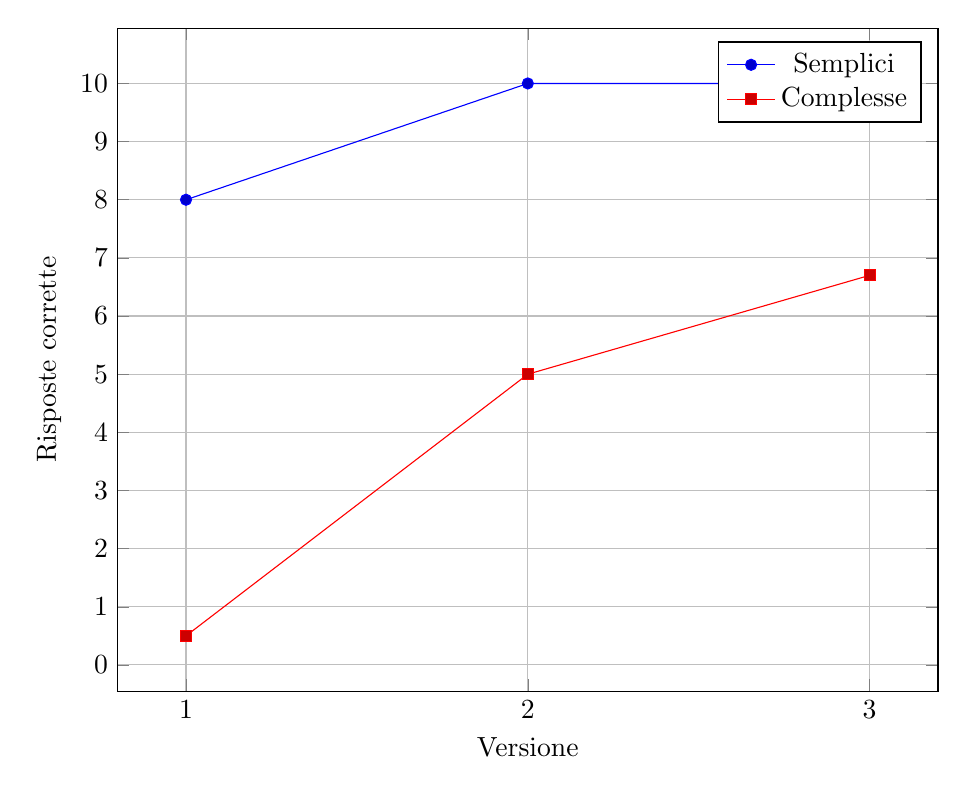
\begin{tikzpicture}
        \centering
        \begin{axis}[
            xlabel={Versione},
            ylabel={Risposte corrette},
            grid=major,
            width=12cm,
            height=10cm,
            xtick={1, 2, 3}, 
            ytick={0, 1, 2, 3, 4, 5, 6, 7, 8, 9, 10}
        ]
        \addplot coordinates {
            (1, 8)
            (2, 10)
            (3, 10)
        };
        \addlegendentry{Semplici}

        \addplot coordinates {
            (1, 0.5)
            (2, 5)
            (3, 6.7)
        };
        \addlegendentry{Complesse}
        
        \end{axis}
    \end{tikzpicture}
    \caption{Grafico risposte corrette su versione - HTML.}

\end{figure}
    
\begin{figure}[H]
    
    \centering
    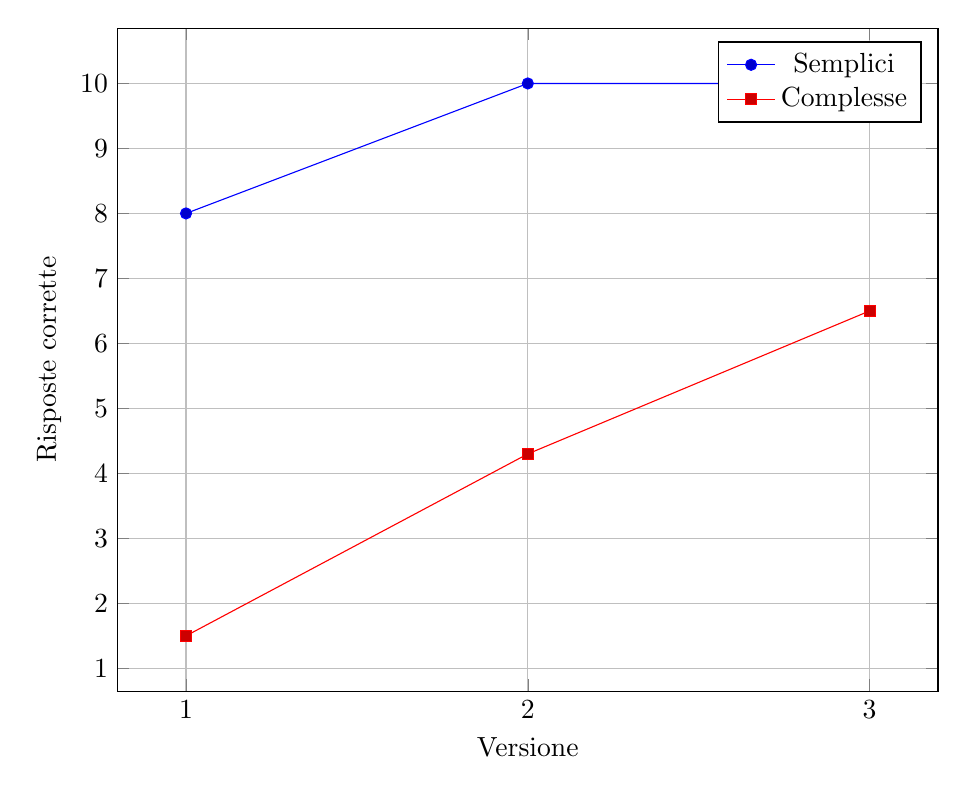
\begin{tikzpicture}
        \centering
        \begin{axis}[
            xlabel={Versione},
            ylabel={Risposte corrette},
            grid=major,
            width=12cm,
            height=10cm,
            xtick={1, 2, 3}, 
            ytick={0, 1, 2, 3, 4, 5, 6, 7, 8, 9, 10}
        ]
        \addplot coordinates {
            (1, 8)
            (2, 10)
            (3, 10)
        };
        \addlegendentry{Semplici}

        \addplot coordinates {
            (1, 1.5)
            (2, 4.3)
            (3, 6.5)
        };
        \addlegendentry{Complesse}
        
        \end{axis}
    \end{tikzpicture}
    \caption{Grafico risposte corrette su versione - Docx.}

\end{figure}

\begin{figure}[H]
    
    \centering
    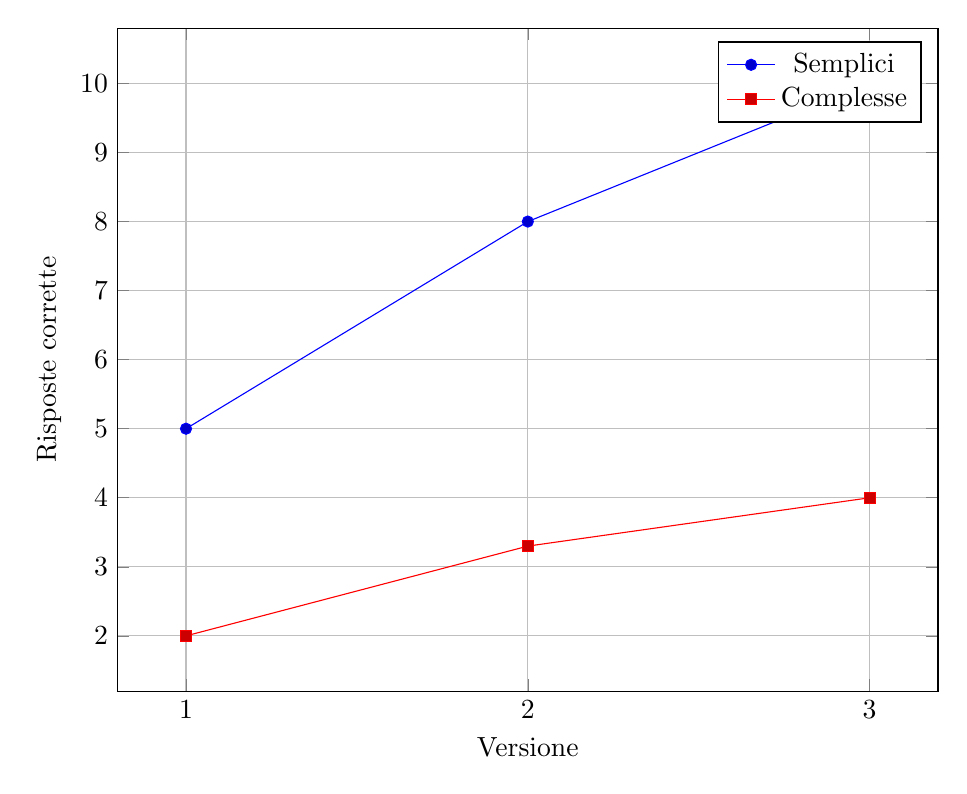
\begin{tikzpicture}
        \centering
        \begin{axis}[
            xlabel={Versione},
            ylabel={Risposte corrette},
            grid=major,
            width=12cm,
            height=10cm,
            xtick={1, 2, 3}, 
            ytick={0, 1, 2, 3, 4, 5, 6, 7, 8, 9, 10}
        ]
        \addplot coordinates {
            (1, 5)
            (2, 8)
            (3, 10)
        };
        \addlegendentry{Semplici}

        \addplot coordinates {
            (1, 2)
            (2, 3.3)
            (3, 4)
        };
        \addlegendentry{Complesse}
        
        \end{axis}
    \end{tikzpicture}
    \caption{Grafico risposte corrette su versione - Pdf.}

\end{figure}



